\documentclass{article}

\usepackage[T1]{fontenc}    %Schriftart des Dokumentes
\usepackage[ngerman]{babel} %Dokumentensprache, hier Deutsch
\usepackage{amsmath, amssymb, stmaryrd} %mathematische Schriftzeichen
\usepackage{graphicx} %Einfügen von Grafiken
\usepackage{wrapfig}
\usepackage{bm}

\setlength{\parindent}{0pt} %Einrückung von Absätzen auf null gesetzt
\setlength{\parskip}{10pt} %Abstand zischen Absätzen auf 10pt gesetzt

\title{Versuch 33: Prismenspektrometer}
\author{Matthias Kuntz}
\date{07.09.2023}

\begin{document}

\maketitle

%-------------------------EINLEITUNG-------------------------
\section{Einleitung}

In diesem Versuch werden die Spektren von Quecksilber-, Helium - und Wasserstofflampen mithilfe eines Prismenspektrometers untersucht. Dabei wird das Quecksilberspektrum als Vorlage genutzt, um eine Winkeldispersionskurve zu erstellen, welche den Ablenkungswinkel des Lichts bei Brechung am Prisma in Abhängigkeit von der Wellenlänge des Lichts angibt. Sinn ist es, mithilfe dieser Eichkurve die Wellenlängen der Spektrallinien der Helium- und Wasserstofflampe zu bestimmen und schlussendlich mit den Spektrallinien der Wasserstofflampe die Rydberg-Konstante zu berechnen.

\subsection{Physikalische Grundlagen}

Hauptbestandteil dieses Versuchs ist das Spektrometer, dessen Aufbau in Abbildung 1 zu sehen ist. Ein Spektrometer ist ein Instrument, mit dem Licht über die Brechung an einem Medium, bei uns ist dies ein Prisma, in seine Spektralfarben und somit Wellenlängen zerlegt werden kann. Ein Prisma ist ein lichtdurchlässiger, von zwei ebenen, nicht parallelen Flächen begrenzter Körper. Die Kante an der sich die beiden Ebenen schneiden heißt brechende Kante und der Winkel zwischen den Ebenen brechender Winkel. Mithilfe des Brechungsgesetz erhält man den gesamten Ablenkungswinkel:

\begin{equation}
    \delta = \alpha_1 - \epsilon + \arcsin{\sqrt{n^2 - \sin{\alpha_1}^2}\sin{\epsilon} - \sin{\alpha_1} \cos{\epsilon}}
\end{equation}

\begin{figure} [h]
\includegraphics[width=10cm]{graphics/abb1.jpg} 
\caption{Skizze eines Spektrometers (oben), Skizze eines Prismas (unten)}
\end{figure}

\newpage

Der minimale Ablenkungswinkel wird erreicht, wenn der Lichtstrahl symmetrisch durch das Prisma verläuft. Dabei gilt:

\begin{equation}
    \begin{split}
        \alpha_{min} &= \alpha_1 = \alpha_2 = \left( \frac{\delta_{min} + \epsilon}{2} \right) \\
        n &= \frac{\sin{(\delta_{min} + \epsilon)/2}}{\sin{\epsilon / 2}}
    \end{split}
\end{equation}

Messungen am Prisma sollten immer bei minimalem Auslenkwinkel durchgeführt werden, da hierbei $\delta$ kaum vom Einfallswinkel $\alpha_1$ abhängt.

Im Allgemeinen hängt der Brechungsindex $n$ aber auch von der Wellenlänge $\lambda$ ab, sodass bei weißem Licht $n(\lambda)$ gilt und der Lichtstrahl spektral zerlegt wird. Somit entsteht die Dispersion, die Aufteilung des Lichts in seine Farben.

Bei diesem Versuch werden Quecksilber-, Helium - und Wasserstofflampen verwendet. Bei diesen wird an das sich im Inneren der Lampe befindende Gas eine Spannung angelegt, die dafür sorgt, dass die Elektronen der Gasteilchen auf ein höheres Energieniveau gebracht werden. Fallen diese dann wieder auf ihr Ursprungsniveau zurück, so werden dabei Photonen emittiert, die stoffabhängige characteristische Wellenlängen besitzen und als Licht der Lampe ausgestrahlt werden. 

Im Spektrometer wird dieses Licht zunächst über ein Spalt mit verändelicher Breite auf die Kollimatorlinse geleitet, die die Lichtstrahlen parallel zueinander auf das Prisma fallen lässt. Nachdem das Licht das Prisma durchläuft, wird es von dem Fernrohr, bestehend aus der Objektivlinse, einem Fadenkreuz im Zwischenbild und der Okularlinse, aufgefangen und kann somit betrachtet werden. 

Zuletzt wird bei diesem Versuch die Balmer-Serie relevant. Sie beschreibt die Folge von Spektrallinien, die von einer Wasserstofflampe emittiert werden. Die Photonen haben hierbei nämlich charakteristische Wellenlängen, mit denen aus der Balmer-Formel die Rydberg-Konstante $R_{\infty}$ bestimmt werden kann:

\begin{equation}
    \begin{split}
        \frac{1}{\lambda} &= R_{\infty} \left( \frac{1}{2^2} - \frac{1}{m^2} \right)
    \end{split}
\end{equation}

Hierbei beschreibt $m$ die Hauptquantenzahl des betreffenden angeregten Zustands. 

\subsection{Versuchsaufbau}

Der Versuchsaufbau ist in Abbildung 1 zu sehen.

Bei diesem Versuch wird zunächst die Quecksilberlampe vor den Spalt des Kollimators gestellt und das Prisma so arretiert, dass der minimale Ablenkwinkel der grünen Linie erzielt wird. Danach werden bei festgehaltener Prismenlage die Ablenkungswinkel von zehn verschiedenen Spektrallinien mit dem Nonius gemessen.

Danach wird die Heliumlampe vor den Spalt gestellt und es werden erneut bei gleicher Prismenlage die Ablenkwinkel für sechs Linien gemessen.

Zuletzt wird die Wasserstofflampe genutzt, um die Ablenkwinkel von insgesamt vier Spektrallinien zu bestimmen.

%---------------VERSUCHSPROTOKOLL MIT MESSDATEN---------------
\newpage

\section{Versuchsprotokoll mit Messdaten}

\includegraphics[width=\textwidth]{graphics/mess1.jpg}
\newpage
\includegraphics[width=\textwidth]{graphics/mess2.jpg}
\newpage
\includegraphics[width=\textwidth]{graphics/mess3.jpg}
\newpage

\addtocounter{table}{3}

%-------------------------AUSWERTUNG-------------------------
\section{Auswertung}

Bevor die Auswertung beginnt eine wichtige Anmerkung: Im Messprotokoll ist versehentlich der falsche Wert für den Ablesefehler $\Delta \delta$ vermerkt worden. Dieser sollte eigentlich bei $\Delta \delta = 0,03^{\circ}$ und nicht bei den angegebenen $\Delta \delta = 0,30^{\circ}$ liegen. Der Wert $\Delta \delta = 0,30^{\circ}$ wäre hier zu groß und ohne Sinn, er würde Fehler der Wellenlänge im dreistelligen Bereich produzieren, die zudem mit der verwendeten grafischen Methode auch gar nicht mehr zu bestimmen wären. Im Folgenden wird also der korrekte Wert von $\Delta \delta = 0,03^{\circ}$ verwendet. 

\subsection{Auswertung des He-Spektrums}

Zunächst wird mithilfe der Daten aus Tabelle 1 die Winkeldispersionskurve $\delta (\lambda)$ des Hg-Spektrums in ein Diagramm eingezeichnet. Dies ist in Abbildung 2 in grüner Farbe zu sehen. Die eingezeichnete Kurve wird im weiteren als Eichkurve verwendet, um die Wellenlängen der gemessenen He-Linien aus Aufgabenteil 4 zu bestimmen. Dazu zeichnet man die in Tabelle 2 gemessenen Winkel in das Diagramm ein, was in Abbildung 2 in blauer Farbe zu erkennen ist und bestimmt die zugehörigen Wellenlängen $\lambda$ mit der Eichkurve. 

Den Fehler der Wellenlänge $\Delta \lambda$ erhält man, indem man den Ablesungsfehler der gemessenen Winkel $\Delta \delta$ des He-Spektrums über und unter die Punkte einzeichnet, bei denen die Winkelwerte auf der Eichkurve liegen und die Wellenlängen bei diesen Winkeln $\delta \pm \Delta \delta$ bestimmt, einmal den Wert vom Fehler oberhalb $\lambda_{oben}$ und den unterhalb $\lambda_{unten}$. Die Differenz zum abgelesenen Wert $\lambda$ vom gemessen $\delta$ gibt dann zwei Werte für Fehler der Wellenlänge an, $\Delta \lambda_{oben}$ und $\Delta \lambda_{unten}$. Dabei wählt man von den beiden Differenzen die Größere als den endgültigen Fehler $\Delta \lambda$. Die Auswertung des He-Sprektrums ist in Tabelle 4 zu sehen, zusammen mit dem im Skript angegeben Literaturwert $\lambda_{lit}$, der im nächsten Schritt zum Vergleich dient.

\begin{table}[h]
\centering
\caption{Auswertung des He-Spektrums sowie Literaturwerte}
\begin{tabular}{c|c|c|c|c|c|c}
\textbf{Nr.} & $\bm{\delta}$ [°] & $\bm{\lambda}$ [nm] & $\bm{\lambda_{oben}}$ [nm] & $\bm{\lambda_{unten}}$ [nm] & $\bm{\Delta \lambda}$ [nm] & $\bm{\lambda_{lit}}$ [nm] \\ \hline
       1   &      1,43     &     661      &      666     &      656     &     5      &     667,8      \\
       2   &      2,00     &     585      &      588     &      581     &     4      &     587,6      \\
       3   &      2,92     &     505      &      507     &      503     &     2      &     501,6      \\
       4   &      3,10     &     493      &      495     &      491     &     2      &     492,2      \\
       5   &      3,45     &     473      &      474     &      471     &     2      &     471,3      \\
       6   &      3,95     &     447      &      449     &      446     &     2      &     447,1     
\end{tabular}
\end{table}

Die bestimmten Fehler $\Delta \lambda$ werden nun noch quadratisch mit dem Ablesefehler des Diagramms $\Delta\lambda_{Dia}$ verrechnet:

\begin{equation}
    \begin{split}
        \Delta \lambda' &= \sqrt{(\Delta \lambda)^2 + (\Delta\lambda_{Dia})^2} \\ \\
        \Delta \lambda'_1 &= 5nm\\
        \Delta \lambda'_2 &= 4nm\\
        \Delta \lambda'_3 &= 2,2nm\\
        \Delta \lambda'_4 &= 2,2nm\\
        \Delta \lambda'_5 &= 2,2nm\\
        \Delta \lambda'_6 &= 2,2nm\\
    \end{split}
\end{equation}

Zum Vergleich mit den Literaturwerten berechnet man die Sigmaabweichungen der sechs Werte $\sigma_1, ..., \sigma_6$ und erhält:

\begin{equation}
    \begin{split}
        \sigma &= \frac{\left| \lambda - \lambda_{lit} \right|}{\left| \Delta \lambda' - \Delta \lambda_{lit} \right|} \\ \\
        \sigma_1 &= 1,4 \\
        \sigma_2 &= 0,7\\
        \sigma_3 &= 1,5\\
        \sigma_4 &= 0,4\\
        \sigma_5 &= 0,8\\
        \sigma_6 &= 0,05
    \end{split}
\end{equation}

Alle Abweichungen liegen also unterhalb der $3\sigma$-Grenze und sind somit nicht signifikant.

\begin{figure} [p]
    \centering
    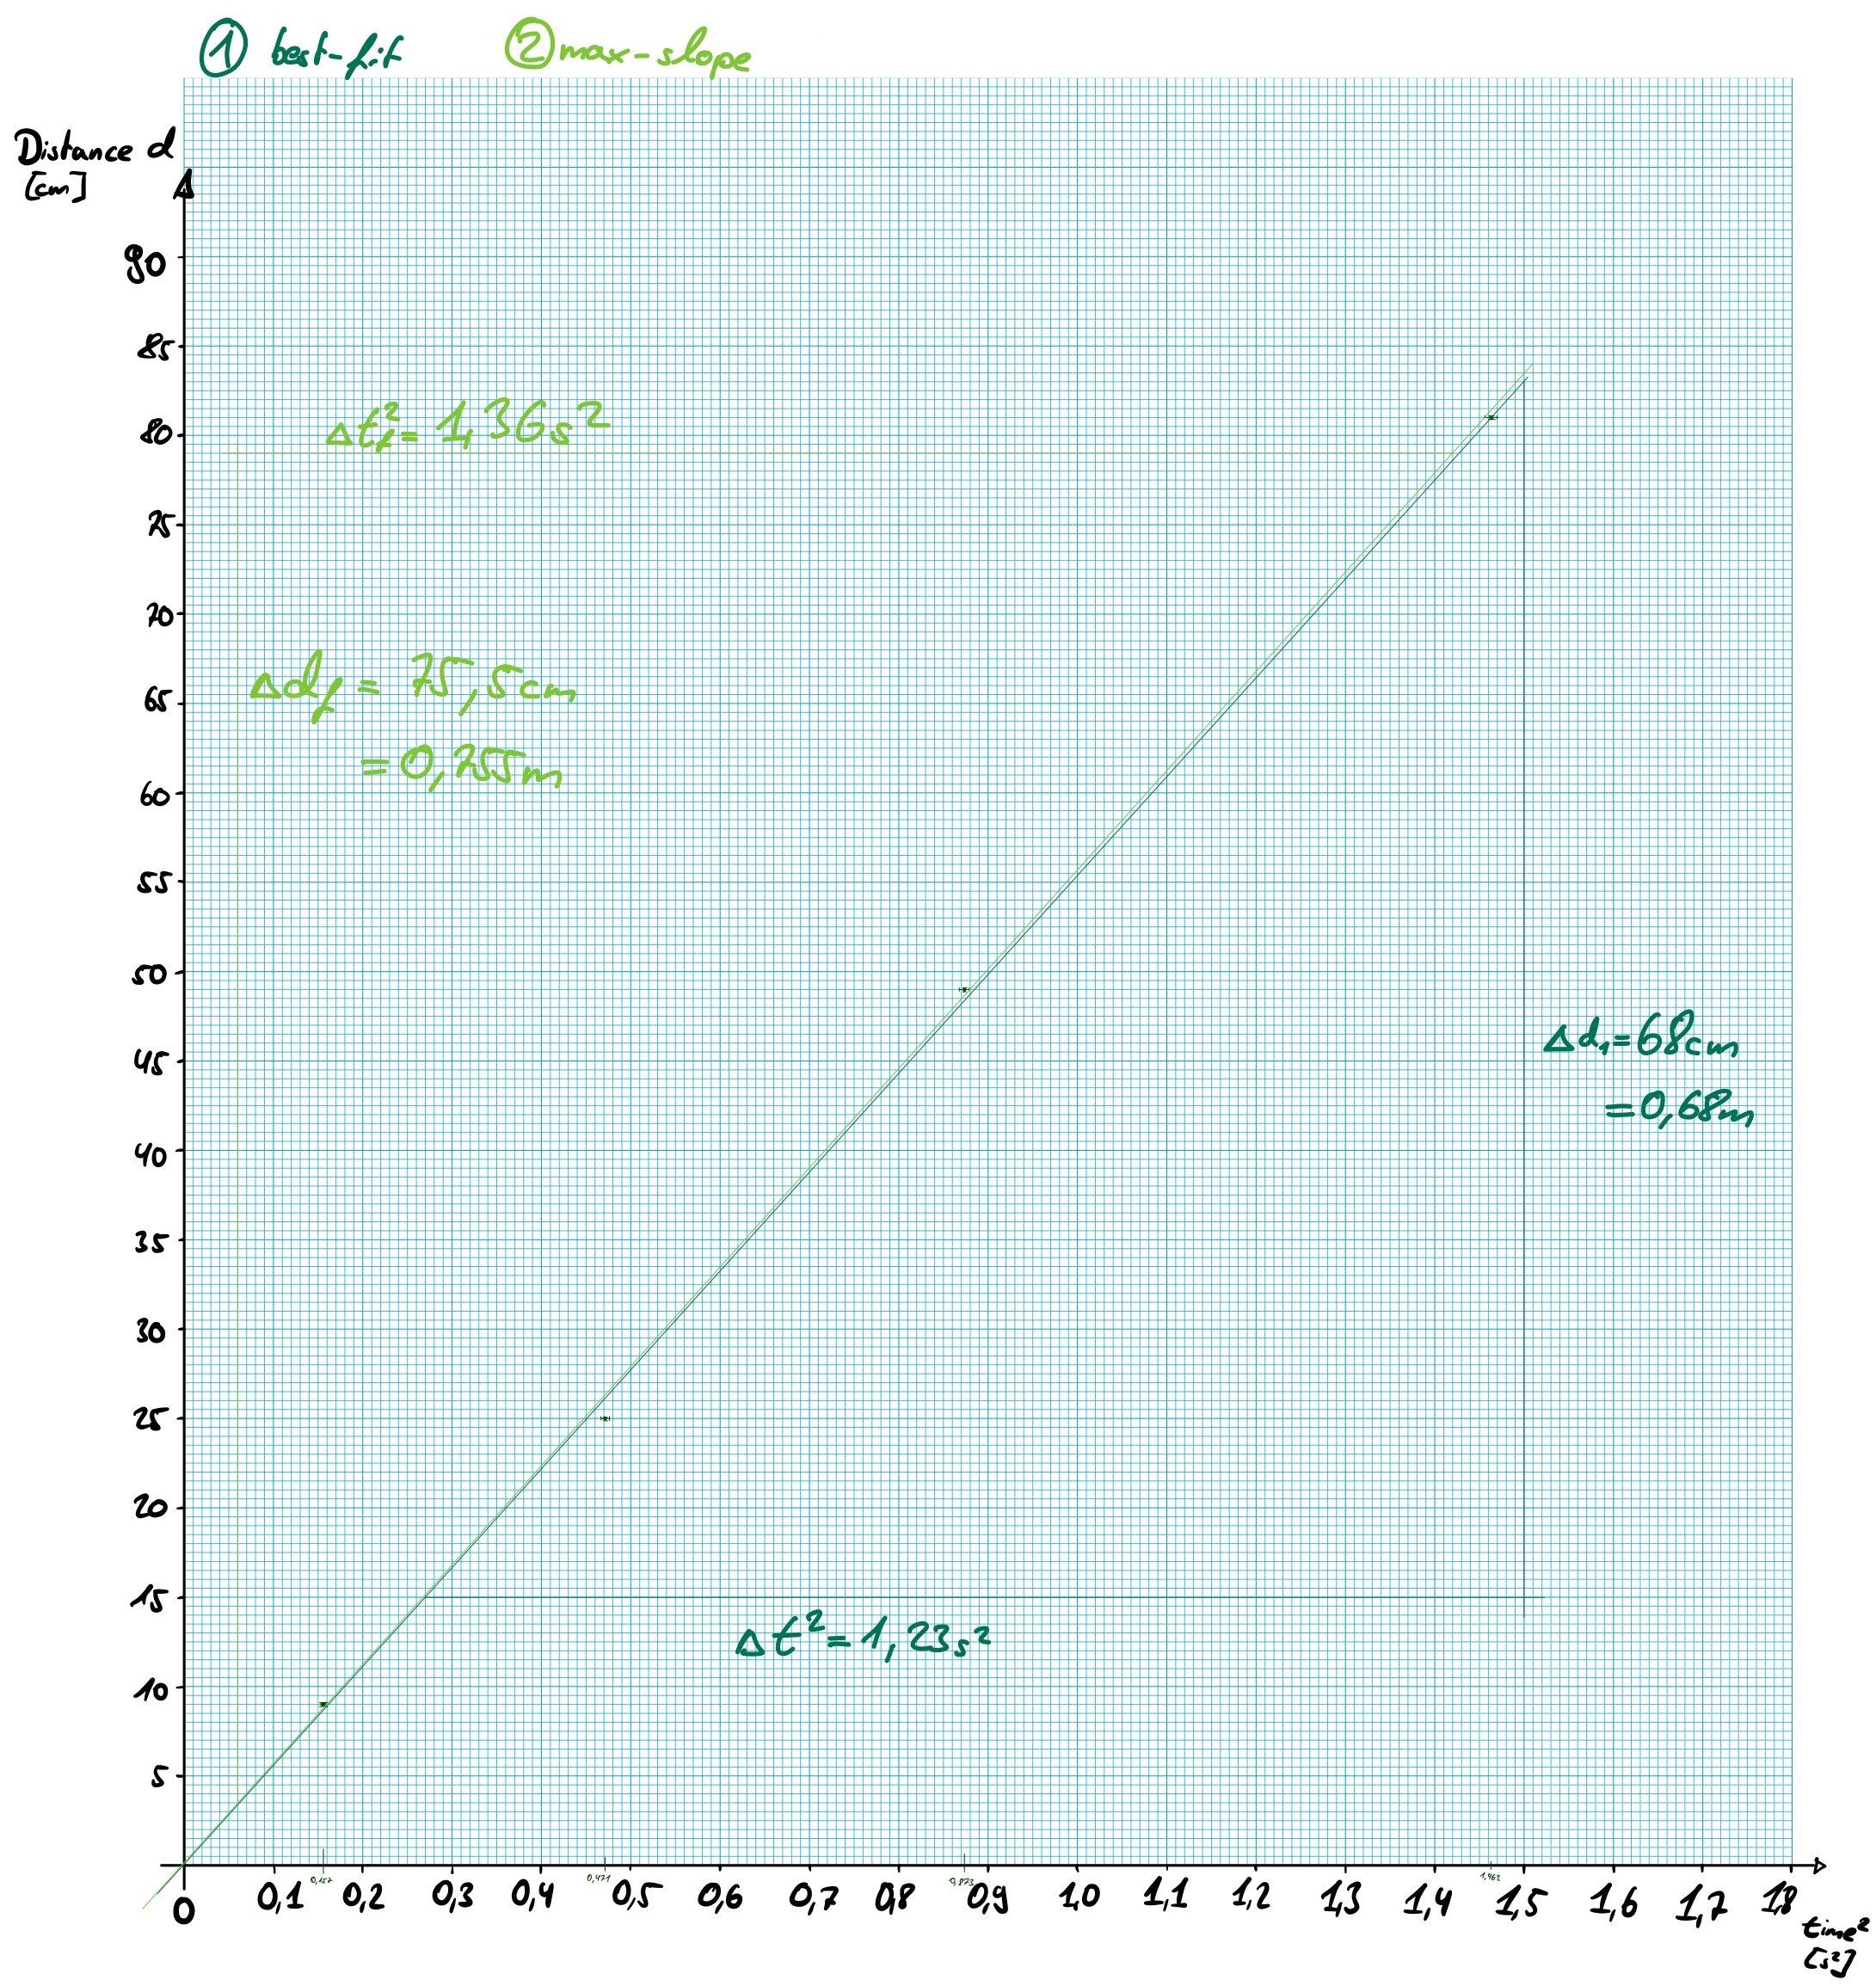
\includegraphics[width=\textwidth]{graphics/dia1.pdf}
    \caption{Diagramm mit Eichkurve und He-Spektrum}
\end{figure}

\newpage

\subsection{Auswertung des H-Spektrums und Bestimmung der Rydberg-Konstante}

Analog werden die gemessenen Winkel für das H-Sprektrum aus Tabelle 3 des Messprotokolls an der Eichkurve eingetragen um so die Wellenlängen zu bestimmen. Die eingezeichneten Winkel sind in Abbildung 3 zu sehen und die Ergebnisse sind in Tabelle 5 abgebildet. Auch hier sind die Literaturwerte dem Skript entnommen.

\begin{table}[h]
\centering
\caption{Auswertung des H-Spektrums sowie Literaturwerte}
\begin{tabular}{c|c|c|c|c|c|c}
\textbf{Nr.} & $\bm{\delta}$ [°] & $\bm{\lambda}$ [nm] & $\bm{\lambda_{oben}}$ [nm] & $\bm{\lambda_{unten}}$ [nm] & $\bm{\Delta \lambda}$ [nm] & $\bm{\lambda_{lit}}$ [nm] \\ \hline
       1   &      1,53     &      645     &      650     &      641     &     5      &     656,3      \\
       2   &      3,22     &      486     &      488     &      484     &     2      &     486,1      \\
       3   &      4,32     &      432     &      433     &      431     &     1      &     434,0      \\
       4   &      1,78     &      611     &      614     &      607     &     4      &     (410,1)   
\end{tabular}
\end{table}

Es ist noch anzumerken, dass wir bei Messwert 4 eine schwache rote Linie vermessen haben. Eigentlich hätte aber eine violette Linie vermessen werden sollen. Somit fällt der Vergleich mit dem Literaturwert hier aus.

Es wird wieder der Ablesefehler des Diagramms verrechnet:

\begin{equation}
    \begin{split}
        \Delta \lambda'_1 &= 5nm\\
        \Delta \lambda'_2 &= 2,2nm\\
        \Delta \lambda'_3 &= 1,4nm\\
        \Delta \lambda'_4 &= 4nm
    \end{split}
\end{equation}

Bei den ersten drei Werten ergeben sich folgende Standartabweichungen:

\begin{equation}
    \begin{split}
        \sigma_1 &= 2,26 \\
        \sigma_2 &= 0,05 \\
        \sigma_3 &= 1,4
    \end{split}
\end{equation}

Somit liegen die drei Abweichungen unterhalb der $3\sigma$-Grenze und sind somit nicht signifikant.

Zuletzt sollen aus den bestimmten Wellenlängen die Rydbergkonstante $R_{\infty}$ mithilfe der Balmer-Formel aus Gleichung 3 bestimmt werden. Für $m$ werden die Werte \{3, 4, 5\} bei $R_{\infty_{1}}$, $R_{\infty_{2}}$ und $R_{\infty_{3}}$ eingesetzt. Da Messung vier nicht die eigentlich gewollte violette Spektrallinie ist, lässt sich hier kein Wert für $m$ finden, weshalb auch diese Berechnung wegfällt. Man erhält:

\begin{equation}
    \begin{split}
        R_{\infty} &= \frac{1}{\lambda} \left( \frac{1}{2^2} - \frac{1}{m^2} \right)^{-1} \\ \\
        R_{\infty_{1}} &= 11162790,70 m^{-1} \\
        R_{\infty_{2}} &= 10973936,90 m^{-1} \\
        R_{\infty_{3}} &= 11022927,7 m^{-1}
    \end{split}
\end{equation}

Die Fehler bestimmt man aus dem Fehlerfortpflanzungsgesetz:

\begin{equation}
    \begin{split}
        \Delta R_{\infty} &= \sqrt{\left( \frac{\partial}{\partial \lambda} \frac{1}{\lambda} \left( \frac{1}{2^2} - \frac{1}{m^2} \right)^{-1} \cdot \Delta \lambda \right)^2} \\ 
        &= \sqrt{\left( \frac{1}{\lambda^2} \left( \frac{1}{2^2} - \frac{1}{m^2} \right)^{-1} \cdot \Delta \lambda \right)^2} \\ \\
        \Delta R_{\infty_{1}} &= 86533,26 m^{-1} \\
        \Delta R_{\infty_{2}} &= 49676,28 m^{-1} \\
        \Delta R_{\infty_{3}} &= 35722,5 m^{-1}
    \end{split}
\end{equation}

Aus den drei Werten wird nun der Mittelwert $\overline{R}_{\infty}$ gebildet und dessen Fehler $\Delta \overline{R}_{\infty}$ mittels Fehlerfortpflanzung bestimmt.

%, welcher dann in quadratischer Addition mit dem Standartfehler des Mittelwerts $\Delta \overline{R}_{\infty_{\sigma}}$ aus der Standartabweichung $\sigma$ den wirklichen Fehler des Mittelwerts $\Delta \overline{R}'_{\infty}$ ergibt:

\begin{equation}
    \begin{split}
        \overline{R}_{\infty} &= \frac{R_{\infty_{1}} + R_{\infty_{2}} + R_{\infty_{3}}}{3} = 11053218,4 m^{-1} \\
        \Delta \overline{R}_{\infty} &= \sqrt{\left( \frac{\Delta R_{\infty_{1}}}{3} \right)^2 + \left( \frac{\Delta R_{\infty_{2}}}{3} \right)^2 + \left( \frac{\Delta R_{\infty_{3}}}{3} \right)^2} = 35326,8 m^{-1} \\ \\
        %\sigma &= 98002,99\\
        %\Delta \overline{R}_{\infty_{\sigma}} &= \frac{\sigma}{\sqrt{3}} = 56582,05 m^{-1} \\ \\
        %\Delta \overline{R}'_{\infty} &= \sqrt{(\Delta \overline{R}_{\infty})^2 + (\Delta \overline{R}_{\infty_{\sigma}})^2} = 66704,7 m^{-1}
        \implies \bm{\overline{R}_{\infty}} &= \bm{(11053218,4 \pm 35326,8) m^{-1}}
    \end{split}
\end{equation}

Zum Vergleich wird der Literaturwert $R_{\infty_{Lit}} = 10973731,568160(21) \frac{1}{m}$ von Wikipedia (Stand: 07.09.2023) genutzt. Man erhält die Standartabweichung:

\begin{equation}
    \sigma = 2,25
\end{equation}

Somit ist die Abweichung innerhalb der $3\sigma$-Umgebung und nicht signifikant

\begin{figure} [p]
    \centering
    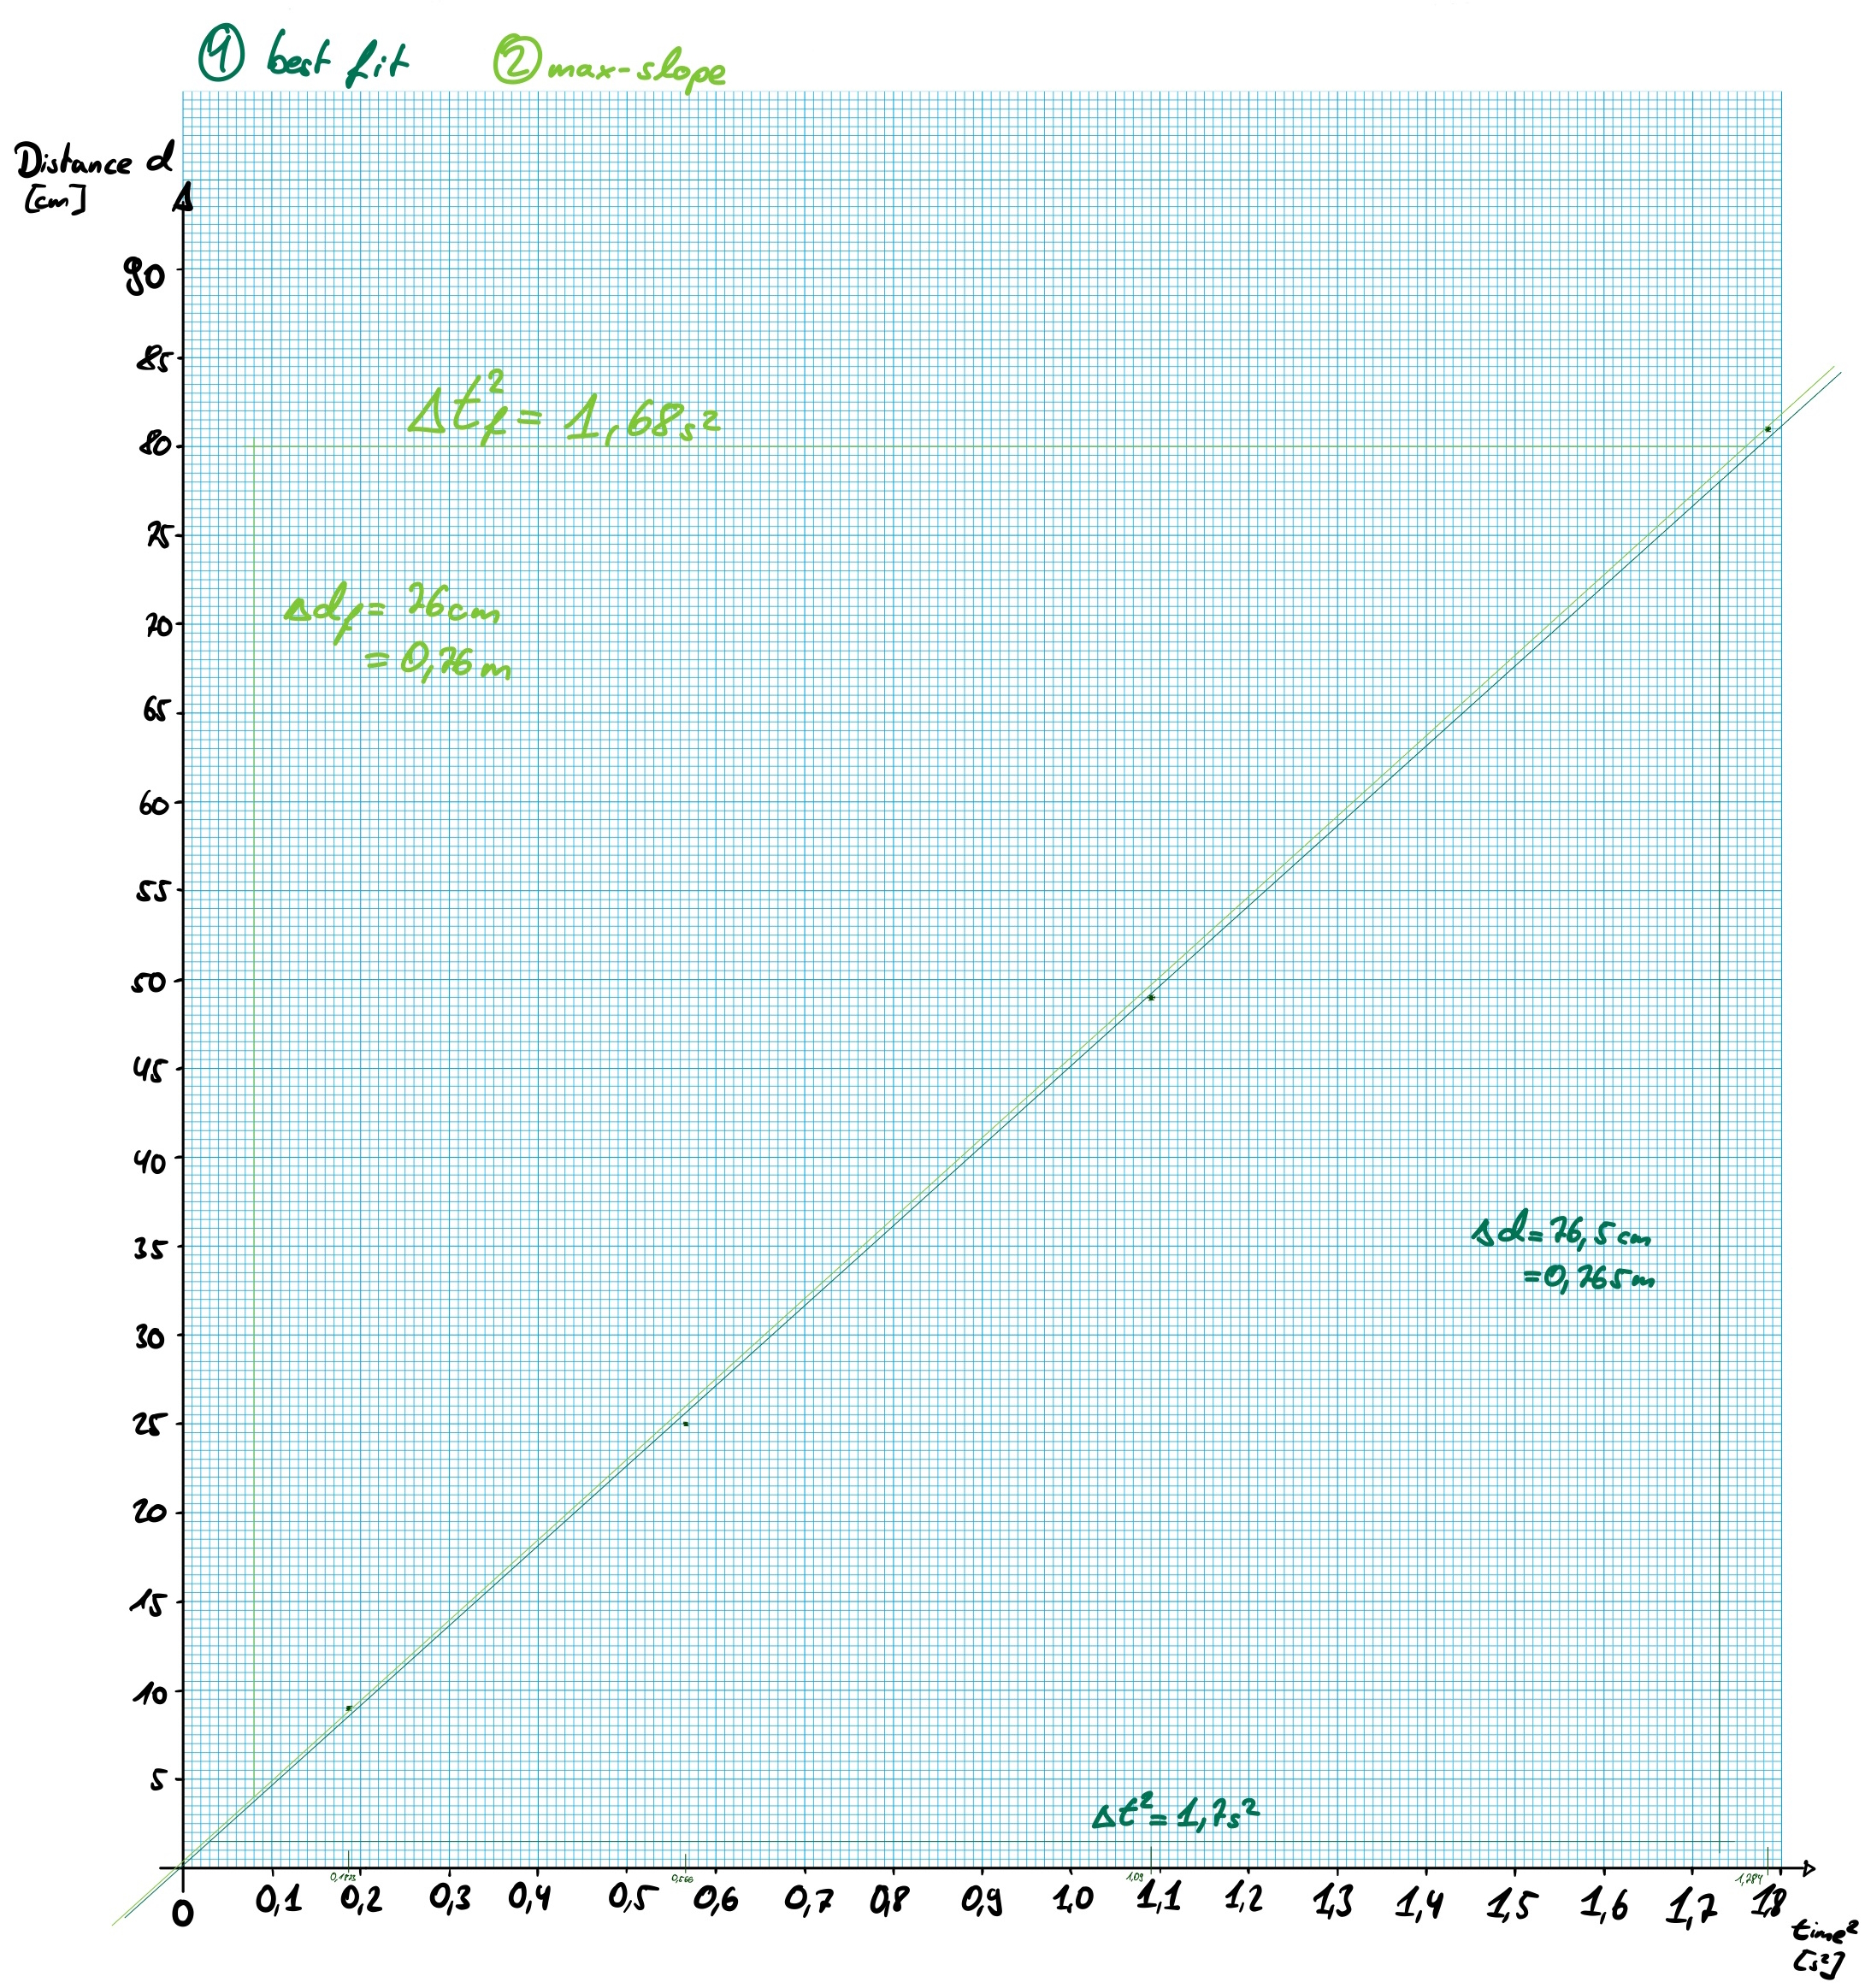
\includegraphics[width=\textwidth]{graphics/dia2.pdf}
    \caption{Diagramm mit Eichkurve und H-Spektrum}
\end{figure}

%---------------PRÄSENTATION DER ENDERGEBNISSE---------------
\newpage

\section{Präsentation der Endergebnisse}

Bei diesem Versuch wurden zunächst die Wellenlängen der im He-Spektrum sichtbaren Spektrallinien mithilfe der Winkeldispersionskurve der Werte der Quecksilberlampe bestimmt. Es wurden folgende Wellenlängen bestimmt, die alle innerhalb der $3\sigma$-Umgebung des Literaturwerts liegen:

\begin{equation}
    \begin{split}
        \bm{\lambda_1} &= \bm{(661 \pm 5) \text{nm}} \\
        \bm{\lambda_2} &= \bm{(585 \pm 4) \text{nm}} \\
        \bm{\lambda_3} &= \bm{(505,0 \pm 2,2) \text{nm}} \\
        \bm{\lambda_4} &= \bm{(493,0 \pm 2,2) \text{nm}} \\
        \bm{\lambda_5} &= \bm{(473,0 \pm 2,2) \text{nm}} \\
        \bm{\lambda_6} &= \bm{(447,0 \pm 2,2) \text{nm}}
    \end{split} 
\end{equation}

Bei der Wasserstofflampe wurden folgende Wellenlängen bestimmt:

\begin{equation}
    \begin{split}
        \bm{\lambda_1} &= \bm{(645 \pm 5) \text{nm}} \\
        \bm{\lambda_2} &= \bm{(486,0 \pm 2,2) \text{nm}} \\
        \bm{\lambda_3} &= \bm{(432,0 \pm 1,4) \text{nm}} \\
        \bm{\lambda_4} &= \bm{(611 \pm 4) \text{nm}}
    \end{split} 
\end{equation}

Von diesen Werten liegen die ersten drei innerhalb der $3\sigma$-Umgebung der Literaturwerte. Aus ihnen wurde die Rydbeckkonstante bestimmt als:

\begin{equation}
    \bm{\overline{R}_{\infty}} = \bm{(11053218,4 \pm 35326,8) m^{-1}}
\end{equation}

Was auch innerhalb der $3\sigma$-Umgebung des Literaturwerts liegt.

%---------------ZUSAMMENFASSUNG UND DISKUSSION---------------
\newpage

\section{Zusammenfassung und Diskussion}

In diesem Versuch wurden die Wellenlängen der Spektrallinien bestimmt, die aus dem Licht von Helium- und Wasserstofflampen durch ein Prismenspektrometer beobachtet werden konnten. Dazu wurde eine Quecksilberlampe genutzt, um mit gegebenen Wellenlängen eine Winkeldispersionskurve zu bestimmen, geeicht auf den minimalen Auslenkwinkel der grünen Spektrallinie. An dieser konnten mit den gemessenen Ablenkwinkeln die Wellenlängen bestimmt werden. Zuletzt wurde mit den Wellenlängen der Wasserstoffspektrallinien die Rydbeck-Konstante bestimmt.

Zunächst lässt sich positiv vermerken, dass alle Berechnungen und Beobachtungen immer erwartete Ergebnisse lieferten. Die Werte ergaben im Vergleich mit den Literaturwerten immer insignifikante Abweichungen innerhalb der $3\sigma$-Umgebung.

Dennoch lässt sich vermerken, dass bei den bestimmten Wellenlängen vier mit erhöhter Sigmaabweichung im Vergleich zu den anderen bestimmt wurden. Dies sind die Werte 1 und 3 des He-Spektrums sowie die Werte 1 und 3 des H-Spektrums. Hierbei ist auffällig, dass die ersten Werte der beiden Spektren jeweils im roten Bereich mit Wellenlängen von etwa 661nm und 645nm liegen. Somit lässt sich vermuten, dass hier entweder ein Fehler unserer Seite beim Bestimmen der Winkel roter Spektrallinien oder eine etwas ungenaue Zeichnung der Eichkurve vorlagen. 

Allgemein lässt sich sagen, dass wohl bei der Eichkurve die größte potenzielle Fehlerquelle liegt. Da diese keine Gerade sondern eine Kurve ist, war es schwer beim Zeichnen die Krümmung und genaue Lage immer so abzuschätzen, dass es am besten passt. Mehr Ausgangswerte, ergo mehr als 10 Wellenlängen des Hg-Spektrums, hätten hierbei sehr geholfen, eine genauere Winkeldispersionskurve zu bestimmen. Zwar haben wir versucht diesem Fehler auch etwas mit der angegebenen Ablesegenauigkeit des Diagramms entgegnzuwirken, jedoch ist diese Abschätzung auch nicht zwangsläufig ausreichend. 

Bei der Bestimmung der Rydbeck-Konstante lässt sich zunächst anmerken, dass wir während des Versuchs die falsche vierte Spektrallinie beobachtet hatten und wir somit nur drei anstatt vier Werte hatten, aus denen wir den Mittelwert berechneten. Somit ist die berechnete Sigmaabweichung mit $\sigma = 2,25$ zwar immer noch innerhalb der $3\sigma$-Umgebung, aber dennoch etwas erhöht sodass eine weitere Messung den berechneten Wert sicherlich verbessert hätte. Ein weiterer Punkt ist hierbei, dass die Nachkommastellen der bestimmen Wellenlängen auf maximal eine gerundet wurden, wodurch Rundungsfehler entstehen, die das Ergebnis möglicherweise genauer erscheinen lassen, als es eigentlich ist. 

Allgemeine Verbesserungspunkte wären zum einen die Justierung des Spektrometers. Hier musste manuell beim Kollimator die Spaltöffnung verschoben werden. Eine Feineinstellung, wie sie beispielsweise mit einem Rädchen beim Fernrohr gegeben war, war somit recht schwierig. Ebenso war die Einstellung des minimalen Ablenkwinkels sicherlich nicht zwangläufig perfekt, da diese auch über eine manuelle Drehung des Prismentischs erfolgte. Zur Verbesserung der Genauigkeit der Eichkurve hätten Computerprogramme geholfen, die nicht nur beim Erstellen von Vorteil wären, sondern auch den Ablesefehler eliminieren könnten.

Zum Schluss lässt sich das Fazit ziehen, dass trotz den genannten potenziellen Fehlerquellen alle Resultate zu Werten ohne signifikante Abweichungen und somit zu sinnvollen Versuchsergebnissen führten.

\end{document}

In diesem Versuch wurden auf zwei verschiedenen Wegen Brennweiten von Linsen bestimmt, diese quantitativ auf die chromatische sowie qualitativ auf die shphärische Aberration untersucht und das Auflösungsvermögen eines Mikroskops bestimmt. 

Dabei lieferten die Berechnungen und Beobachtungen fast immer erwartete Ergebnisse. Bei den ersten drei Teilen ergaben die Werte im Vergleich miteinander immerzu Sinn und passten mit unserem physikalischen Verständnis überein. 

Bei Teil Eins lässt sich das mit der berechneten Sigmaabweichung von $\sigma = 0,63$ zwischen dem grafisch und rechnerisch bestimmten Wert für $f$ begründen, die sogar noch unterhalb der $1\sigma$-Grenze liegt. 

Beim zweiten Teil gab es zwar keine Angaben zum Vergleich, der berechnete Wert von $f = (12,13 \pm 0,04)cm$ erscheint im Kontext des Versuchs aber als sinnvoll und passt zu den Ergebnissen von Teil drei, bei dem wie erwartet die Brennweite für rotes Licht länger als die für blaues Licht berechnet wurde und der Wert ohne Farbfilter zwischen den beiden liegt. Physikalisch lässt sich diese Beobachtung damit begründen, dass blaues Licht eine kürzere Wellenlänge hat und somit stärker gebrochen wird. Bei rotem Licht ist dann genau das Gegenteil der Fall. \\
Die Beobachtung der sphärischen Aberration erfolgte hier dann nur qualitiativ, ergab aber, dass der Abstand $d$ im Schnitt bei der Ringblende größer und bei der Lochblende kleiner wird. Das sorgt im Endeffekt für eine kleinere Brennweite bei der Lochblende im Vergleich zur Ringblende was bestätigt, dass achsenferne Lichtbündel tatsächlich stärker gebrochen werden als achsennahe. 

Nur bei Aufgabenteil Vier ergab sich ein nicht vorhergesehenes Ergebnis. Hier wurde die Gitterkonstante als $l_{Gitter} = (0,099 \pm 0,010) mm$ und das Auflösungsvermögen als $G_{min} = (0,116 \pm 0,024)mm$ bestimmt, was zum Quotienten $\frac{l_{Gitter}}{G_{min}} = 0,85$ führte, der eigentlich größer als 1 sein sollte. Fehlerquellen könnten hier eine falsche Messung des Strichabstands beim Zwischenbild, eine ungenaue Einstellung der Bildweite von 25cm oder ein Messfehler bei Bestimmung der Spaltbreite sein. Auch ist die etwas sperrige Bedienung des Schiebers zur Einstellung der Spaltbreite hier erwähnenswert, dieser blieb nämlich gerne mal etwas hängen und motivierte somit eventuell zu psychologischen Fehlern und Fehleinschätzungen. Zudem war insgesamt die Abschätzung, ab wann die senkrechten Strukturen des Gitters nicht mehr zu erkennen waren, recht schwierig. Dennoch lässt sich erwähenen, dass es theoretisch Werte größer als 1 gibt, die, vorausgesetzt sie haben einen ähnlichen Fehler wie der bestimmte Wert $\Delta \frac{l_{Gitter}}{G_{min}}$, noch innerhalb der $1\sigma$-Umgebung von unserem Quotienten liegen. Die Abweichung ist also theoretisch hier nicht signifikant, aber das Ergebnis, dass $l_{Gitter}$ kleiner ist als $G_{min}$, bleibt nicht richtig. 

Während des Versuchs wurden noch nach dem gleichen Verfahren wie im vierten Teil die Spaltbreiten bei rotem und blauen Licht qualitativ betrachtet. Man konnte feststellen, dass die Spaltbreite beim blauen Licht etwas kleiner und beim roten Licht etwas größer wird. 

Allgemein lassen sich trotz der weitgehend vereinbaren Ergebnisse noch folgende Kritikpunkte und potenzielle Fehlerquellen nennen.

Zunächst sind allgemeine Messfehler, Ablesefehler und Gerätefehler zu nennen. Während Messfehler bei uns nicht aufgefallen sind und wir Ablesefehler im allgemeinen gut abschätzen konnten, gab es bei diesem Versuch keine Angaben über Gerätefehler der bereitgestellten Materialien, wie z.B. der Brennweite der Linse, wo nur der von uns abgeschätzte Ablesefehler der Skala verwendet werden konnte. 

Eine weitere nennenswerte potentielle Fehlerquelle war der Schirm, auf dem in den ersten drei Versuchsteilen das Bild betrachtet wurde. Dieser war nämlich dadurch, dass sich die Plastikbeschichtung auf dem Metall etwas zu lösen begann, an manchen Stellen sichtbar gewölbt. Wie im Messprotokoll erwähnt haben wir hierfür einen etwas größeren Fehler abgeschätzt, dennoch ist unsere Abschätzung sicherlich nicht zwangsweise perfekt.   

Des Weitern lässt sich vermerken, dass die Abschätzung der richtigen Position, bei der das Bild scharf ist, nach persönlichem Ermessen erfolgte und somit nicht perfekt sein kann, da der Unterschied zwischen einem scharfen und einem gerade so nicht mehr scharfen Bild häufig schwer zu differenzieren war. 

Zum Schluss lässt sich das Fazit ziehen, dass trotz den genannten potenziellen Fehlerquellen alle Resultate, bis auf die Thematisierten in Teil Vier, zu Werten ohne signifikante Abweichungen sowie zu Beobachtungen, die nicht im Konflikt mit unseren Erwartungen stehen würden, und somit zu sinnvollen Versuchsergebnissen führten.